\documentclass[crop,tikz]{standalone}
\usepackage{tikz}
\usetikzlibrary{calc}
\usetikzlibrary{positioning}
\begin{document}
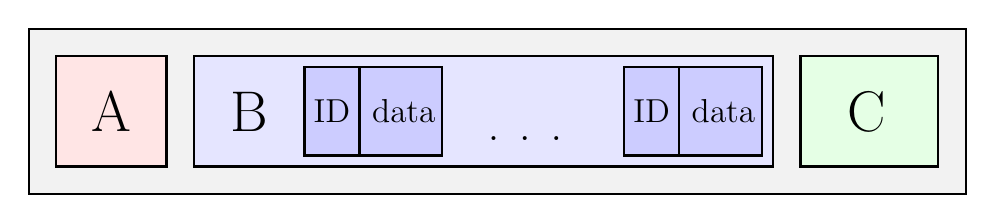
\begin{tikzpicture}[scale=0.07,rotate=0]
		
	%Frame
	\draw[thick, draw=black, fill=gray!10] (0,0) rectangle (170,30);

	%Segments
	%A
	\draw[thick, draw=black, fill=red!10] (5,5) rectangle (25,25);
	\node at (15,15) {\huge A};

	%B
	\draw[thick, draw=black, fill=blue!10] (30,5) rectangle (135,25);
	\node at (40,15) {\huge B};
	
	%B1
	\draw[thick, draw=black, fill=blue!20] (50,7) rectangle (60,23);
	\draw[thick, draw=black, fill=blue!20] (60,7) rectangle (75,23);
	\node at (55,15) {\large ID};
	\node at (68,15) {\large data};
	
	\node at (90,10) {\LARGE . . .};
	
	%Bn
	\draw[thick, draw=black, fill=blue!20] (118,7) rectangle (133,23);
	\draw[thick, draw=black, fill=blue!20] (108,7) rectangle (118,23);
	\node at (113,15) {\large ID};
	\node at (126,15) {\large data};

	%C
	\draw[thick, draw=black, fill=green!10] (140,5) rectangle (165,25);
	\node at (152,15) {\huge C};
	
\end{tikzpicture}
\end{document}